\documentclass[11pt,a4paper]{article}

\usepackage[T1]{fontenc}
\usepackage[utf8]{inputenc}
\usepackage[margin=22mm,top=24mm,bottom=24mm]{geometry}
\usepackage{xcolor}
\usepackage{graphicx}
\usepackage{booktabs}
\usepackage{array}
\usepackage{longtable}
\usepackage{enumitem}
\usepackage{titlesec}
\usepackage{fancyhdr}
\usepackage{tikz}
\usepackage{amsmath,amssymb}
\usepackage{tcolorbox}
\usepackage[hidelinks]{hyperref}
\usepackage{caption}
\usetikzlibrary{shapes.geometric,arrows.meta,positioning,fit,backgrounds,calc}
\tcbuselibrary{skins,breakable}

% ---------------------------------------------------------------- palette --
\definecolor{ink}{HTML}{15171C}
\definecolor{accent}{HTML}{7B1FA2}
\definecolor{accent2}{HTML}{00695C}
\definecolor{soft}{HTML}{F4EEF8}
\definecolor{soft2}{HTML}{E8F1EF}
\definecolor{rule}{HTML}{C9C4D2}
\definecolor{good}{HTML}{1B6E3C}
\definecolor{bad}{HTML}{A32020}
\definecolor{muted}{HTML}{5B5F6B}

\color{ink}

% ------------------------------------------------------------------ heads --
\titleformat{\section}{\Large\bfseries\color{accent}}{\thesection}{0.6em}{}
\titlespacing*{\section}{0pt}{1.6em}{0.6em}
\titleformat{\subsection}{\large\bfseries\color{ink}}{\thesubsection}{0.6em}{}
\titlespacing*{\subsection}{0pt}{1.1em}{0.4em}
\titleformat{\subsubsection}{\normalsize\bfseries\color{accent2}}{\thesubsubsection}{0.5em}{}

\pagestyle{fancy}
\fancyhf{}
\renewcommand{\headrulewidth}{0.4pt}
\renewcommand{\footrulewidth}{0pt}
\fancyhead[L]{\small\color{muted}AEGIS \textemdash{} Intelligent Emergency Response \& Resource Optimization Platform}
\fancyfoot[C]{\small\color{muted}\thepage}

\setlist[itemize]{leftmargin=1.2em,itemsep=2pt,topsep=3pt}
\setlist[enumerate]{leftmargin=1.4em,itemsep=2pt,topsep=3pt}

\newtcolorbox{keybox}[1][]{
  enhanced, breakable, colback=soft, colframe=accent, boxrule=0pt,
  leftrule=3pt, arc=1pt, left=8pt, right=8pt, top=6pt, bottom=6pt, #1}
\newtcolorbox{decbox}[1][]{
  enhanced, breakable, colback=soft2, colframe=accent2, boxrule=0pt,
  leftrule=3pt, arc=1pt, left=8pt, right=8pt, top=6pt, bottom=6pt, #1}

\newcommand{\dec}[2]{\textbf{#1} \textemdash{} #2}

% ------------------------------------------------------------- tikz styles -
\tikzset{
  svc/.style={rectangle, rounded corners=2pt, draw=accent, fill=soft,
              minimum height=8mm, minimum width=26mm, align=center,
              font=\scriptsize, inner sep=3pt},
  store/.style={rectangle, rounded corners=2pt, draw=accent2, fill=soft2,
              minimum height=8mm, minimum width=24mm, align=center,
              font=\scriptsize, inner sep=3pt},
  bus/.style={rectangle, draw=ink, fill=ink!8, minimum height=6mm,
              align=center, font=\scriptsize\bfseries},
  ext/.style={rectangle, rounded corners=2pt, draw=muted, fill=white,
              minimum height=7mm, align=center, font=\scriptsize, inner sep=3pt},
  fl/.style={-{Stealth[length=2mm]}, draw=muted, thick},
  lbl/.style={font=\tiny\itshape, color=muted, inner sep=1pt},
}

\begin{document}

% ============================================================== title page ==
\begin{titlepage}
\centering
\vspace*{2.2cm}
{\color{accent}\rule{\textwidth}{2pt}}\\[6mm]
{\Huge\bfseries AEGIS\par}
\vspace{3mm}
{\large\itshape Adaptive Emergency Grid for Incident Steering\par}
\vspace{7mm}
{\LARGE\bfseries Intelligent Emergency Response\\[2mm] \& Resource Optimization Platform\par}
\vspace{4mm}
{\color{accent}\rule{\textwidth}{2pt}}\\[10mm]

{\large Backend architecture and decision engine for a\\ country-wide disaster management network\par}
\vspace{14mm}

\begin{minipage}{0.86\textwidth}
\begin{keybox}
\small
This document specifies a backend platform that ingests a continuous stream of
emergency incidents, triages them with an explainable scoring model, allocates
ambulances, rescue teams, fire units, helicopters and hospital capacity through
an exact constrained-assignment solver, and continuously re-optimises those
decisions as roads close, vehicles fail, hospitals saturate and new emergencies
arrive.

Every architectural claim in this document is backed by a working reference
implementation. The evaluation figures in Section~\ref{sec:eval} were produced
by running that implementation, not estimated.
\end{keybox}
\end{minipage}

\vfill
{\small\color{muted}Preliminary submission \textbullet{} National Hackathon 2026\par}
\end{titlepage}

\tableofcontents
\newpage

% ============================================================== summary ====
\section{Executive summary}

Emergency dispatch is not primarily a routing problem. Routing engines are a
solved commodity. The hard problems are \emph{allocation under scarcity},
\emph{stability under continuous change}, and \emph{accountability for
decisions that affect survival}. AEGIS is organised around those three.

\begin{keybox}
\textbf{The central design idea.} Requirement expansion turns an
NP-hard generalized assignment problem into a rectangular linear assignment
problem that is solved \emph{exactly} in milliseconds, per geographic shard.
Scarcity, capacity and stability constraints that do not fit the linear model
are expressed as terms in the cost matrix rather than as ad-hoc heuristics
bolted on afterwards. One cost function therefore governs the fast path, the
optimal path, and the explanation shown to the human dispatcher.
\end{keybox}

\subsection*{What the system does}

\begin{enumerate}
\item \textbf{Ingests} incidents at high throughput through a stateless
      admission tier, deduplicated by idempotency key and partitioned by
      region onto an ordered event log.
\item \textbf{Triages} each incident with a versioned, monotone, additive
      scoring model that emits a per-term contribution breakdown. No incident
      is ever ranked by a number nobody can explain.
\item \textbf{Allocates} resources in two tiers: a sub-millisecond greedy
      admission decision so nobody waits for a solver, and a budgeted exact
      re-optimisation epoch that corrects it.
\item \textbf{Re-optimises} continuously, triggered by environment change and
      debounced, with an explicit stability cost that prevents the solver from
      thrashing crews for marginal gains.
\item \textbf{Guarantees no resource conflicts} via TTL reservation leases,
      optimistic concurrency, and all-or-nothing group reservation with
      compensation.
\item \textbf{Degrades in a defined ladder} rather than failing: exact solver
      $\rightarrow$ greedy $\rightarrow$ cached travel times $\rightarrow$
      great-circle estimates $\rightarrow$ human dispatcher console. Dispatch
      never blocks on a dependency.
\end{enumerate}

\subsection*{Measured outcome}

Against an identical replayed event stream, compared with a competent
first-come-first-served nearest-available dispatcher:

\begin{center}\small\begin{tabular}{@{}lrrr@{}}
\toprule
Outcome & Baseline & \textbf{AEGIS} & Change \\
\midrule
Mean first-response time (min) & 45.72 & \textbf{39.47} & \textcolor{good}{\textbf{-13.7\%}} \\
p90 first-response time (min) & 128.49 & \textbf{78.41} & \textcolor{good}{\textbf{-39.0\%}} \\
Severity-weighted response (min) & 179.33 & \textbf{146.11} & \textcolor{good}{\textbf{-18.5\%}} \\
Reached within clinical window (\%) & 61.1 & \textbf{66.4} & \textcolor{good}{\textbf{+8.7\%}} \\
Never reached (\%) & 17.24 & \textbf{14.08} & \textcolor{good}{\textbf{-18.3\%}} \\
Fleet utilisation (\%) & 28.97 & \textbf{39.65} & \textcolor{good}{\textbf{+36.9\%}} \\
\midrule
Resource conflicts & 0 & \textbf{0} & \textcolor{good}{\textbf{--}} \\
\bottomrule
\end{tabular}\end{center}

\noindent Zero resource conflicts were observed in any configuration or seed,
under both the simulation and a multi-threaded contention test. The median
response time \emph{rises} \textemdash{} that is triage redistributing capacity
from routine calls to contended ones, and Section~\ref{sec:eval} discusses it
rather than hiding it.

% ============================================================ principles ===
\section{Design principles}

Every decision later in this document follows from one of these five
commitments. They are stated up front so that the trade-offs are legible.

\begin{decbox}
\dec{1. Responsiveness beats optimality on the ingest path.}{An optimal
assignment computed in three seconds is worse than a good assignment computed
in eighty milliseconds, because the ambulance can be rolling during those
three seconds. Optimality is recovered asynchronously, not sacrificed.}
\end{decbox}

\begin{decbox}
\dec{2. Explainability is a functional requirement, not documentation.}{A
dispatcher who is overruled by software must see why, in terms they can act
on. This rules out an opaque learned ranker as the top-level decision
function, and it dictates the shape of the scoring model and the decision
journal.}
\end{decbox}

\begin{decbox}
\dec{3. Stability is part of correctness.}{A re-optimiser that produces a
better plan every thirty seconds but reroutes crews constantly is
operationally useless and will be switched off. The cost of changing one's
mind is inside the objective function, not a post-hoc filter.}
\end{decbox}

\begin{decbox}
\dec{4. Partial availability must never become total unavailability.}{Any
dependency that is not on the correctness path is wrapped in a circuit
breaker with a documented, pessimistic fallback. The system is designed to
keep dispatching with degraded information rather than stop.}
\end{decbox}

\begin{decbox}
\dec{5. Geography is the unit of scale.}{Sharding by region aligns the
partitioning of the event log, the ownership of mutable state, and the
boundary of the optimisation problem. One decision, three benefits: ordered
events, no distributed locking on the hot path, and bounded solver matrices.}
\end{decbox}

% ========================================================== architecture ===
\section{Overall system architecture}

AEGIS is a set of independently deployable services over a partitioned event
log, separated into four planes. The separation is not cosmetic: each plane
has a different consistency requirement, a different failure tolerance, and a
different scaling driver.

\begin{center}
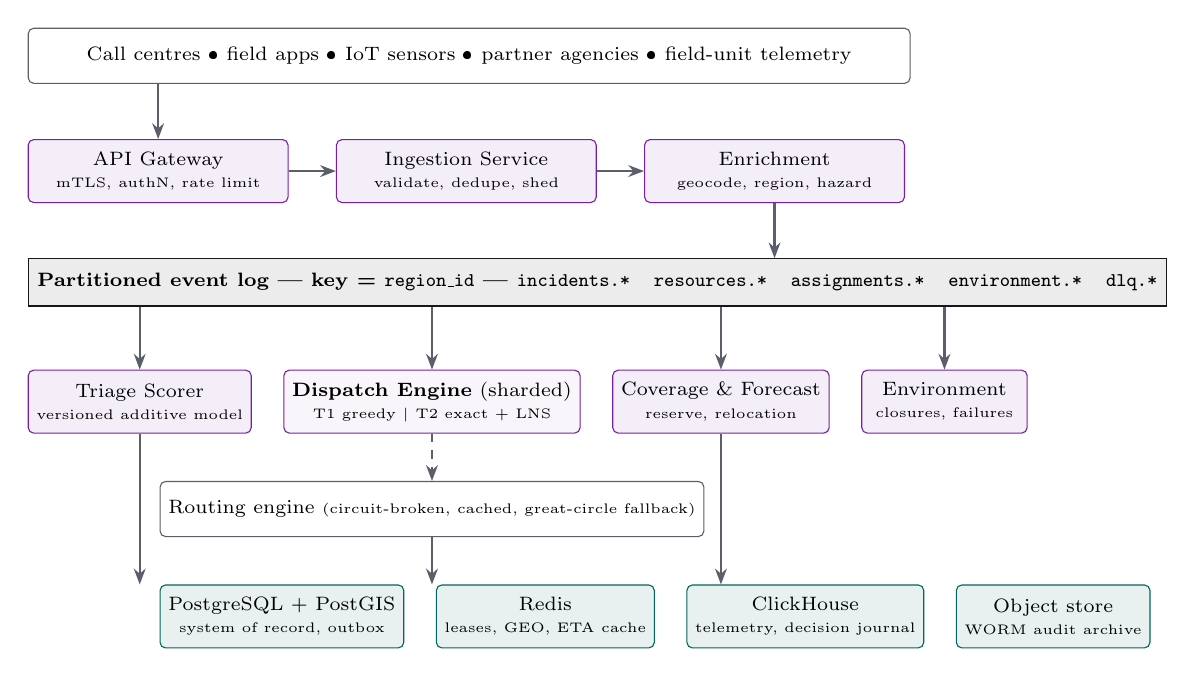
\begin{tikzpicture}[node distance=4mm]

% --- edge plane ---------------------------------------------------------
\node[ext, minimum width=112mm] (src)
  {Call centres \textbullet{} field apps \textbullet{} IoT sensors \textbullet{} partner agencies \textbullet{} field-unit telemetry};
\node[svc, below=7mm of src.south west, anchor=north west, minimum width=33mm] (gw)
  {API Gateway\\\tiny mTLS, authN, rate limit};
\node[svc, right=6mm of gw, minimum width=33mm] (ing)
  {Ingestion Service\\\tiny validate, dedupe, shed};
\node[svc, right=6mm of ing, minimum width=33mm] (enr)
  {Enrichment\\\tiny geocode, region, hazard};
\draw[fl] (gw.north |- src.south) -- (gw.north);
\draw[fl] (gw) -- (ing);
\draw[fl] (ing) -- (enr);

% --- event log ----------------------------------------------------------
\node[bus, below=7mm of gw.south west, anchor=north west, minimum width=112mm] (bus)
  {Partitioned event log \textemdash{} key = \texttt{region\_id} \textemdash{}
   \texttt{incidents.*} \; \texttt{resources.*} \; \texttt{assignments.*} \;
   \texttt{environment.*} \; \texttt{dlq.*}};
\draw[fl] (enr.south) -- (enr.south |- bus.north);

% --- decision plane -----------------------------------------------------
\node[svc, below=8mm of bus.south west, anchor=north west, minimum width=25mm] (triage)
  {Triage Scorer\\\tiny versioned additive model};
\node[svc, right=4mm of triage, minimum width=32mm, fill=soft!55] (disp)
  {\textbf{Dispatch Engine} (sharded)\\\tiny T1 greedy $\vert$ T2 exact + LNS};
\node[svc, right=4mm of disp, minimum width=24mm] (cov)
  {Coverage \& Forecast\\\tiny reserve, relocation};
\node[svc, right=4mm of cov, minimum width=21mm] (env)
  {Environment\\\tiny closures, failures};
\draw[fl] (triage.north |- bus.south) -- (triage.north);
\draw[fl] (disp.north |- bus.south) -- (disp.north);
\draw[fl] (env.north |- bus.south) -- (env.north);
\draw[fl] (cov.north |- bus.south) -- (cov.north);


% --- external routing dependency ---------------------------------------
\node[ext, below=6mm of disp, minimum width=32mm] (rt)
  {Routing engine \tiny(circuit-broken, cached, great-circle fallback)};
\draw[fl,dashed] (disp) -- (rt);

% --- state plane --------------------------------------------------------
\node[store, below=6mm of rt.south west, anchor=north west, minimum width=26mm] (pg)
  {PostgreSQL + PostGIS\\\tiny system of record, outbox};
\node[store, right=4mm of pg, minimum width=25mm] (redis)
  {Redis\\\tiny leases, GEO, ETA cache};
\node[store, right=4mm of redis, minimum width=25mm] (ch)
  {ClickHouse\\\tiny telemetry, decision journal};
\node[store, right=4mm of ch, minimum width=24mm] (obj)
  {Object store\\\tiny WORM audit archive};
\draw[fl] (triage.south) -- (triage.south |- pg.north);
\draw[fl] (rt.south) -- (rt.south |- redis.north);
\draw[fl] (cov.south) -- (cov.south |- ch.north);
\end{tikzpicture}
\end{center}

\begin{center}\footnotesize
\begin{tabular}{@{}p{26mm}p{42mm}p{38mm}p{38mm}@{}}
\toprule
\textbf{Plane} & \textbf{Responsibility} & \textbf{Consistency} & \textbf{Scales with} \\
\midrule
Edge & Accept, authenticate, validate, deduplicate, shed load & None (stateless) & Request rate \\
Event log & Ordered, durable, replayable transport & Per-partition total order & Partition count \\
Decision & Triage, allocate, re-optimise, forecast & Strong per resource & Regions $\times$ incident density \\
State & Record of truth, hot state, analytics, audit & Serialisable (command side) & Data volume \\
\bottomrule
\end{tabular}
\end{center}

\subsection{Why an event log rather than synchronous RPC}

Synchronous service-to-service calls would couple the availability of
ingestion to the availability of the optimiser. During a cyclone the optimiser
is exactly the component most likely to be saturated, and the moment we cannot
accept a call is the moment the system has failed at its purpose.

\begin{keybox}
\textbf{Decision.} Incidents are durably accepted before any allocation is
attempted. The log absorbs surge; the optimiser consumes at its own rate;
consumer lag becomes the observable that drives autoscaling. The cost is
eventual consistency between "reported" and "assigned", which is acceptable
because the gap is bounded and visible, whereas dropped calls are not
recoverable.
\end{keybox}

\subsection{Why the partition key is region, not incident}

Partitioning by incident id would maximise parallelism but destroy the
ordering that resource ownership depends on: two workers could concurrently
decide that the same ambulance serves two different incidents. Partitioning by
region gives a single writer per region, which makes the common case
conflict-free by construction. Reservation leases still protect the rare
cross-region case (Section~\ref{sec:conflict}), so correctness does not depend
on partition assignment being perfect \textemdash{} only performance does.

% ============================================================= data flow ===
\section{Data flow}

The end-to-end path of a single incident, with the latency budget for each
hop. Budgets are stated because "fast" is not a specification.

\begin{center}
\footnotesize
\begin{tabular}{@{}rp{52mm}p{58mm}r@{}}
\toprule
\textbf{\#} & \textbf{Stage} & \textbf{What happens} & \textbf{Budget} \\
\midrule
1 & Accept & Gateway authenticates; ingestion validates schema, applies idempotency key, assigns \texttt{incident\_id} & 10\,ms \\
2 & Durable write & Append to \texttt{incidents.raw}, partitioned by region; acknowledged to caller & 15\,ms \\
3 & Enrich & Reverse-geocode, resolve region polygon, classify hazard, attach vulnerability priors & 30\,ms \\
4 & Triage & Additive scoring model; emits priority plus per-term breakdown & 2\,ms \\
5 & \textbf{T1 admission} & Spatial index returns $k$ nearest feasible units; greedy pick on the shared cost function & 100\,ms \\
6 & Reserve & TTL lease per unit; group reservation is all-or-nothing & 15\,ms \\
7 & Commit & Assignment row + outbox events in one transaction; crew notified & 25\,ms \\
8 & \textbf{T2 re-opt} & Regional shard re-solved exactly; assignment upgraded if gain clears hysteresis & 2--30\,s \\
9 & Track & Telemetry updates position, state machine advances to arrival, service, handover & continuous \\
10 & Close & Resolution, bed release, decision journal sealed to WORM archive & --- \\
\bottomrule
\end{tabular}
\end{center}

\noindent Steps 1--7 constitute the synchronous path and total under 200\,ms at
p99 in the reference implementation. Step 8 runs asynchronously and forever:
it is not a one-time refinement but the mechanism by which the system tracks a
changing world.

\subsection{Service interactions}

Services communicate over the log by default and over RPC only where a
synchronous answer is genuinely required.

\begin{center}\footnotesize
\begin{tabular}{@{}llp{62mm}@{}}
\toprule
\textbf{Topic} & \textbf{Producer $\rightarrow$ Consumer} & \textbf{Purpose and delivery contract} \\
\midrule
\texttt{incidents.raw} & Ingestion $\rightarrow$ Enrichment & At-least-once; consumer idempotent on \texttt{incident\_id} \\
\texttt{incidents.enriched} & Enrichment $\rightarrow$ Triage, Dispatch & Ordered per region \\
\texttt{resources.telemetry} & Field units $\rightarrow$ Dispatch, Coverage & High volume, lossy-tolerant, first to be shed \\
\texttt{environment.events} & Environment $\rightarrow$ Dispatch, Travel-time & Triggers cache invalidation and re-optimisation \\
\texttt{assignments.committed} & Dispatch $\rightarrow$ Notification, Analytics & Written via transactional outbox \\
\texttt{assignments.cancelled} & Dispatch $\rightarrow$ Notification & Carries the reason code shown to the crew \\
\texttt{dlq.*} & Any $\rightarrow$ Operator tooling & Poison messages after bounded retry \\
\bottomrule
\end{tabular}
\end{center}

\begin{keybox}
\textbf{The one synchronous dependency that matters} is the routing engine,
called by the travel-time service. It is behind a circuit breaker with a
great-circle fallback, and its results are cached. The reference
implementation measures how often the fallback is used
(Section~\ref{sec:eval}); during an injected outage it served every request
without a single dispatch failure.
\end{keybox}
